\documentclass[12pt, letterpaper]{article}

% Packages
\usepackage[utf8]{inputenc}
\usepackage{geometry}
\usepackage{graphicx}
\usepackage{listings}
\usepackage{xcolor}
\usepackage{float}
\usepackage{enumitem}
\usepackage{array}
\usepackage{amsmath}
\usepackage{tikz}
\usepackage{hyperref}

\usetikzlibrary{positioning}

% Page Layout
\geometry{margin=1in}

% Code listing style
\definecolor{codebg}{rgb}{0.95,0.95,0.95}
\definecolor{codegreen}{rgb}{0,0.5,0}
\definecolor{codegray}{rgb}{0.5,0.5,0.5}
\definecolor{codepurple}{rgb}{0.58,0,0.82}

\lstdefinestyle{pythonstyle}{
    backgroundcolor=\color{codebg},
    commentstyle=\color{codegreen},
    keywordstyle=\color{blue},
    numberstyle=\tiny\color{codegray},
    stringstyle=\color{codepurple},
    basicstyle=\ttfamily\scriptsize,
    breakatwhitespace=false,
    breaklines=true,
    captionpos=b,
    keepspaces=true,
    numbers=left,
    numbersep=5pt,
    showspaces=false,
    showstringspaces=false,
    showtabs=false,
    tabsize=4,
    language=Python,
    frame=single,
}

\lstdefinestyle{outputstyle}{
    basicstyle=\ttfamily\tiny,
    breaklines=true,
    frame=single,
    numbers=none,
    backgroundcolor=\color{codebg},
    xleftmargin=0.5em,
    framexleftmargin=0.3em,
    aboveskip=0.5em,
    belowskip=0.5em,
}

% TikZ styles
\tikzset{
    netnode/.style={
        circle, draw, fill=white,
        minimum size=10mm, font=\bfseries,
        line width=0.6pt
    },
    edgelabel/.style={
        font=\small, fill=white, inner sep=2pt
    }
}

% Header Information
\title{\textbf{Homework 6}}
\author{Yousef Alaa Awad}
\date{\today}

% Custom Formatting Commands
\newcommand{\lab}[1]{\section*{Lab #1}}
\newcommand{\task}[1]{\subsection*{Task #1}}
\newcommand{\question}[1]{\noindent\textbf{Question: }#1\par\vspace{0.5em}}
\newcommand{\answer}{\noindent\textbf{Answer:}\par\vspace{0.5em}}

\begin{document}

\maketitle

% ============================================================================
% LAB 1: DV ROUTING ALGORITHM
% ============================================================================
\lab{1: DV Routing Algorithm}

\task{1-1: DV Routing for a 2$\times$2 Node Network}

The 2$\times$2 network contains 4 nodes (a, b, c, d) connected as a grid:

\begin{center}
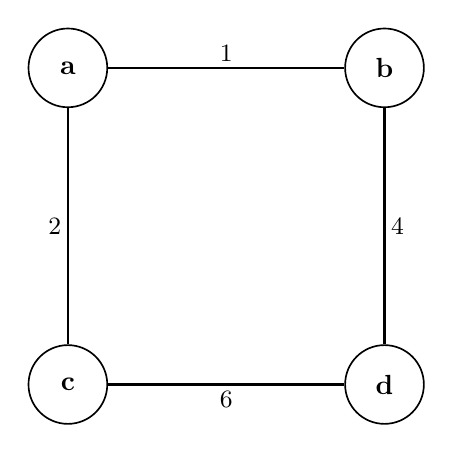
\begin{tikzpicture}[node distance=3cm]
    \node[netnode] (a) {a};
    \node[netnode, right=of a] (b) {b};
    \node[netnode, below=of a] (c) {c};
    \node[netnode, right=of c] (d) {d};

    \draw[thick] (a) -- node[edgelabel, above] {1} (b);
    \draw[thick] (a) -- node[edgelabel, left]  {2} (c);
    \draw[thick] (b) -- node[edgelabel, right] {4} (d);
    \draw[thick] (c) -- node[edgelabel, below] {6} (d);
\end{tikzpicture}
\end{center}

The DV algorithm converges in \textbf{3 iterations}. Initial DV tables contain only direct neighbor costs (non-neighbors set to $\infty$). With each iteration, nodes exchange distance vectors with neighbors and update using the Bellman-Ford equation:
$D_x(y) = \min_v\{c(x,v) + D_v(y)\}$.

\lstinputlisting[style=outputstyle, caption={Task 1-1 Output}, firstline=1, lastline=38]{dv_output.txt}


\task{1-2: DV Routing for a 4$\times$4 Node Network}

The 4$\times$4 grid network has 16 nodes (0--15) with randomly generated edge weights in $[1, 10]$:

\begin{center}
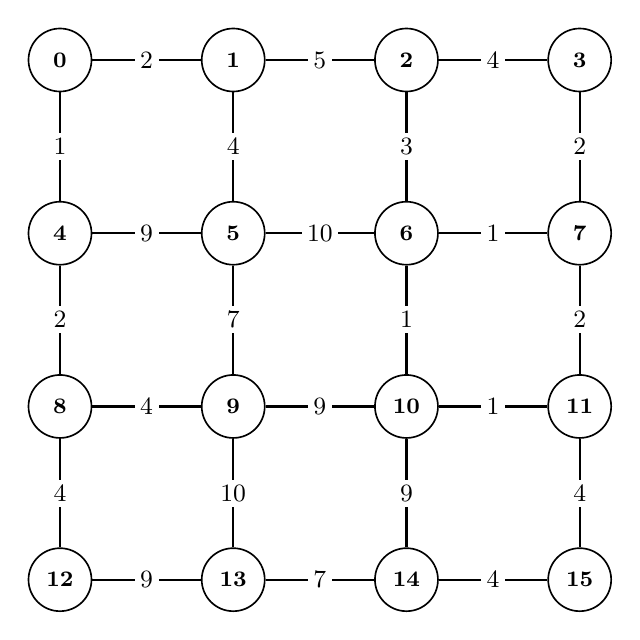
\begin{tikzpicture}[every node/.style={font=\small}]
    % Nodes
    \foreach \r in {0,...,3} {
        \foreach \c in {0,...,3} {
            \pgfmathtruncatemacro{\id}{\r*4+\c}
            \node[netnode, minimum size=8mm, font=\footnotesize\bfseries]
                (n\id) at (\c*2.2, -\r*2.2) {\id};
        }
    }
    % Horizontal edges (weights from seed=42)
    \draw[thick] (n0)  -- node[edgelabel] {2}  (n1);
    \draw[thick] (n1)  -- node[edgelabel] {5}  (n2);
    \draw[thick] (n2)  -- node[edgelabel] {4}  (n3);
    \draw[thick] (n4)  -- node[edgelabel] {9}  (n5);
    \draw[thick] (n5)  -- node[edgelabel] {10} (n6);
    \draw[thick] (n6)  -- node[edgelabel] {1}  (n7);
    \draw[thick] (n8)  -- node[edgelabel] {4}  (n9);
    \draw[thick] (n9)  -- node[edgelabel] {9}  (n10);
    \draw[thick] (n10) -- node[edgelabel] {1}  (n11);
    \draw[thick] (n12) -- node[edgelabel] {9}  (n13);
    \draw[thick] (n13) -- node[edgelabel] {7}  (n14);
    \draw[thick] (n14) -- node[edgelabel] {4}  (n15);
    % Vertical edges
    \draw[thick] (n0)  -- node[edgelabel] {1}  (n4);
    \draw[thick] (n1)  -- node[edgelabel] {4}  (n5);
    \draw[thick] (n2)  -- node[edgelabel] {3}  (n6);
    \draw[thick] (n3)  -- node[edgelabel] {2}  (n7);
    \draw[thick] (n4)  -- node[edgelabel] {2}  (n8);
    \draw[thick] (n5)  -- node[edgelabel] {7}  (n9);
    \draw[thick] (n6)  -- node[edgelabel] {1}  (n10);
    \draw[thick] (n7)  -- node[edgelabel] {2}  (n11);
    \draw[thick] (n8)  -- node[edgelabel] {4}  (n12);
    \draw[thick] (n9)  -- node[edgelabel] {10} (n13);
    \draw[thick] (n10) -- node[edgelabel] {9}  (n14);
    \draw[thick] (n11) -- node[edgelabel] {4}  (n15);
\end{tikzpicture}
\end{center}

The DV algorithm converges in \textbf{7 iterations} (with seed=42).

\vspace{0.5em}
\lstinputlisting[style=outputstyle, caption={Task 1-2 Output}]{dv_output.txt}

\subsection*{Questions}

\question{For an $N \times N$ network, how many iterations does it require to complete the DV routing?}

\answer
The DV algorithm converges in at most $D$ iterations, where $D$ is the network diameter in hops. For an $N \times N$ grid, $D = 2(N-1)$. So convergence requires at most $\mathbf{2(N-1)}$ iterations (plus one to confirm stability). For a $2 \times 2$ grid: 2--3 iterations. For a $4 \times 4$ grid: 6--7 iterations.

\question{In Figure 2, what could be the potential impact if one specific link becomes disconnected (i.e., its distance becomes infinite)?}

\answer
Adjacent nodes set the link cost to $\infty$ and trigger reconvergence. If the failed link was on a shortest path, the \textbf{count-to-infinity problem} may occur---nodes slowly increment distance estimates before stabilizing. Traffic reroutes through longer alternative paths for increased latency. A single link failure cannot partition a grid (alternative paths always exist), but multiple failures could.

\pagebreak
% ============================================================================
% LAB 2: PROTECTION STRATEGIES
% ============================================================================
\lab{2: Protection Strategies}

\task{2-1: CRC-8 and SEC-DED Encoding}

For the input value \texttt{0xFA7816EB87CC0911} (64 bits):

\begin{itemize}
    \item \textbf{CRC-8} (polynomial 0x107: $x^8 + x^2 + x + 1$): The computed 8-bit CRC is \texttt{0x5B} (binary: \texttt{01011011}). The encoded output is \texttt{0xFA7816EB87CC09115B} (72 bits).
    \item \textbf{SEC-DED} (Hamming code + overall parity): 7 Hamming parity bits + 1 overall parity bit = 8 parity bits, producing a 72-bit codeword. The encoded output is \texttt{0x17D3605B570F981211}.
\end{itemize}

\lstinputlisting[style=outputstyle, caption={Task 2-1 Output}, firstline=1, lastline=18]{protection_output.txt}

\task{2-2: Error Detection Evaluation}

Each error type was injected 1,000,000 times, and the detection rates for CRC-8 and SEC-DED are summarized below:

\begin{center}
\begin{tabular}{|l|c|c|}
\hline
\textbf{Error Type} & \textbf{CRC Rate (\%)} & \textbf{SEC-DED Rate (\%)} \\ \hline
A single-bit error       & 100.0000 & 100.0000 \\ \hline
Two random-bit errors    & 100.0000 & 100.0000 \\ \hline
Three random-bit errors  & 100.0000 & 100.0000 \\ \hline
An 8-bit burst error     & 100.0000 & $\sim$97.61 \\ \hline
A 16-bit burst error     & $\sim$99.61 & $\sim$98.62 \\ \hline
\end{tabular}
\end{center}

\textbf{Observations:}
\begin{itemize}
    \item CRC-8 detects 100\% of burst errors up to 8 bits long (matching the CRC degree), and $\sim$99.6\% of 16-bit bursts.
    \item SEC-DED detects 100\% of 1, 2, and 3-bit errors (by design, it corrects single errors and detects double errors; triple errors are also detected in practice due to the overall parity bit). Burst errors are less reliably detected.
\end{itemize}

\subsection*{Questions}

\question{What is the concept of Hamming distance? Why cannot SEC-DED correct two errors?}

\answer
\textbf{Hamming distance} is the number of bit positions in which two codewords differ. The minimum Hamming distance $d_{\min}$ of a code determines its capabilities: detecting $t$ errors requires $d_{\min} \geq t+1$; correcting $t$ errors requires $d_{\min} \geq 2t+1$.

SEC-DED has $d_{\min} = 4$, so it can correct 1 error and detect up to 2. It \textbf{cannot correct two errors} because a word with 2 errors may be equidistant from two valid codewords, making it impossible to determine the original.

\question{Typically, SEC-DED is implemented using combinational circuits, while CRC is implemented using sequential circuits. Is it possible to implement CRC using combinational circuits?}

\answer
\textbf{Yes.} CRC is polynomial division in GF(2) using only XOR and shifts. For a fixed-length input, this can be unrolled into a combinational XOR-gate tree. However, it requires many gates, has long propagation delay, and is hardwired to one input length---unlike a sequential LFSR, which is compact and handles arbitrary-length data. Combinational CRC is sometimes used in high-throughput, fixed-frame applications.

\pagebreak
% ============================================================================
% SOURCE CODE
% ============================================================================
\section*{Source Code}

\subsection*{Lab 1: DV Routing (\texttt{dv\_routing.py})}
\lstinputlisting[style=pythonstyle, caption={DV Routing Algorithm Implementation}]{dv_routing.py}

\pagebreak
\subsection*{Lab 2: Protection Strategies (\texttt{protection.py})}
\lstinputlisting[style=pythonstyle, caption={CRC-8 and SEC-DED Implementation}]{protection.py}

\end{document}
